\begin{figure}[H]
  \begin{center}
	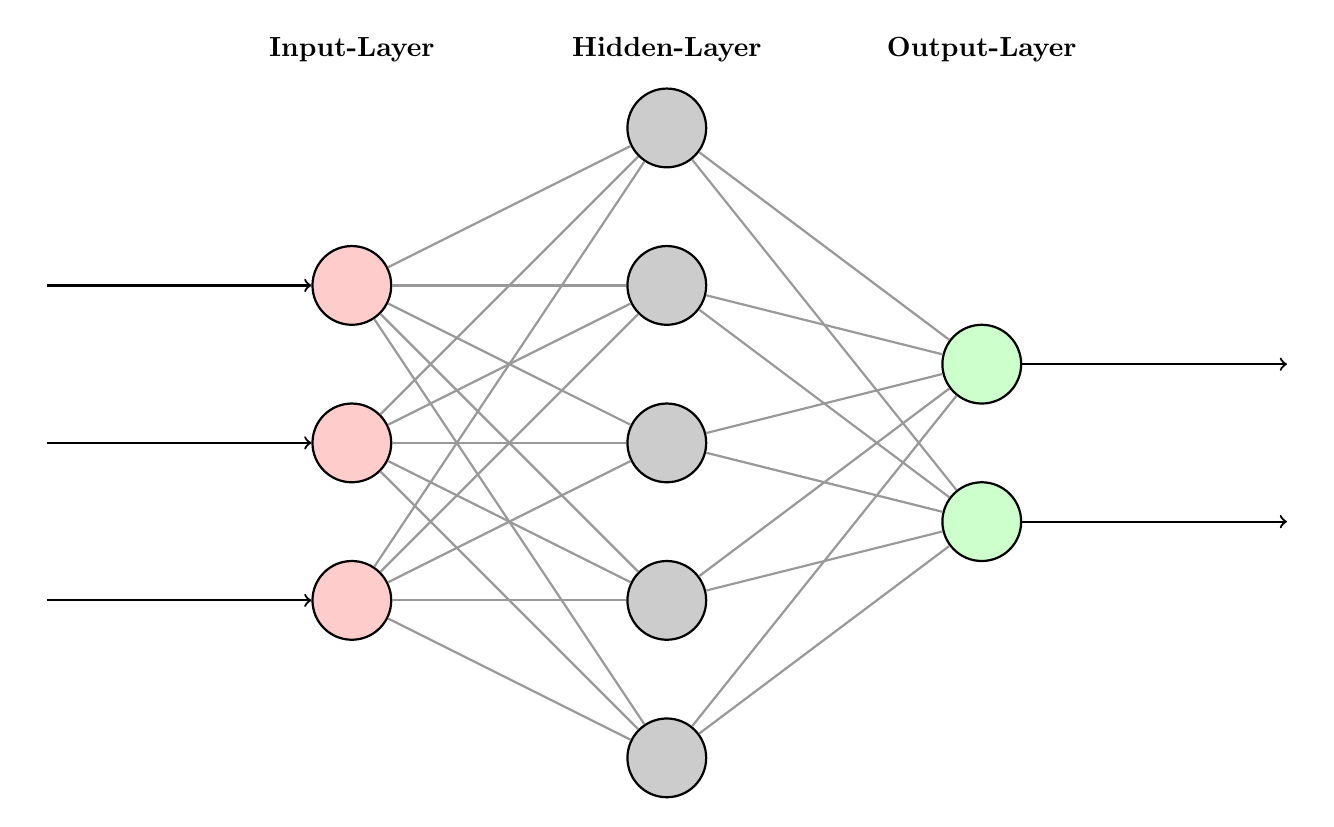
\begin{tikzpicture}[%
    dot/.style={circle,draw,thick,minimum size = 1cm}
  ]
		\node at(-4,5) {\textbf{Input-Layer}};
		\node at(0,5) {\textbf{Hidden-Layer}};
		\node at(4,5) {\textbf{Output-Layer}};

		\node at(8,1) (oo1) {};
		\node at(8,-1) (oo2) {};

		\node at (4,1) [dot,fill=green!20] (o1) {}
			edge[->,thick] (oo1);
		\node at (4,-1) [dot,fill=green!20] (o2) {}
			edge[->,thick] (oo2);

		\node at (0,4) [dot,fill=black!20] (h1) {}
			edge[thick,black!40] (o1)
			edge[thick,black!40] (o2);
		\node at (0,2) [dot,fill=black!20] (h2) {}
			edge[thick,black!40] (o1)
			edge[thick,black!40] (o2);
		\node at (0,0) [dot,fill=black!20] (h3) {}
			edge[thick,black!40] (o1)
			edge[thick,black!40] (o2);
		\node at (0,-2) [dot,fill=black!20] (h4) {}
			edge[thick,black!40] (o1)
			edge[thick,black!40] (o2);
		\node at (0,-4) [dot,fill=black!20] (h5) {}
			edge[thick,black!40] (o1)
			edge[thick,black!40] (o2);

		\node at (-4,2) [dot,fill=red!20] (i1) {}
			edge[thick,black!40] (h1)
			edge[thick,black!40] (h2)
			edge[thick,black!40] (h3)
			edge[thick,black!40] (h4)
			edge[thick,black!40] (h5);
		\node at (-4,0) [dot,fill=red!20] (i2) {}
			edge[thick,black!40] (h1)
			edge[thick,black!40] (h2)
			edge[thick,black!40] (h3)
			edge[thick,black!40] (h4)
			edge[thick,black!40] (h5);
		\node at (-4,-2) [dot,fill=red!20] (i3) {}
			edge[thick,black!40] (h1)
			edge[thick,black!40] (h2)
			edge[thick,black!40] (h3)
			edge[thick,black!40] (h4)
			edge[thick,black!40] (h5);

		\node at(-8,2) (ii1) {}
			edge[->,thick] (i1);
		\node at(-8,0) (ii2) {}
			edge[->,thick] (i2);
		\node at(-8,-2) (ii3) {}
			edge[->,thick] (i3);
	\end{tikzpicture}
  \end{center}
  \caption{Neural network with hidden layer}
  %\label{snn}
\end{figure}
